\documentclass[11pt]{beamer}
\usetheme{Warsaw}
\usepackage[utf8]{inputenc}
\usepackage{amsmath}
\usepackage{amsfonts}
\usepackage{amssymb}
\usepackage{graphicx}
\author{Gianluca Rossi}
\title{A primer on Bayesian Hierarchical modelling}
%\setbeamercovered{transparent} 
%\setbeamertemplate{navigation symbols}{} 
%\logo{} 
%\institute{} 
\date{January 18, 2017} 
%\subject{} 
\begin{document}

\begin{frame}
	\titlepage
\end{frame}

%%%%%%%%%%%%%%%%%%%%%%%%%%

\begin{frame}
	\tableofcontents
\end{frame}

%%%%%%%%%%%%%%%%%%%%%%%%%%

\section{A primer on Bayes' Theorem}
\subsection{The Bayes' Theorem}
\begin{frame}
	\frametitle{Let's start with some art}
%	\framesubtitle{}
	\begin{figure}
		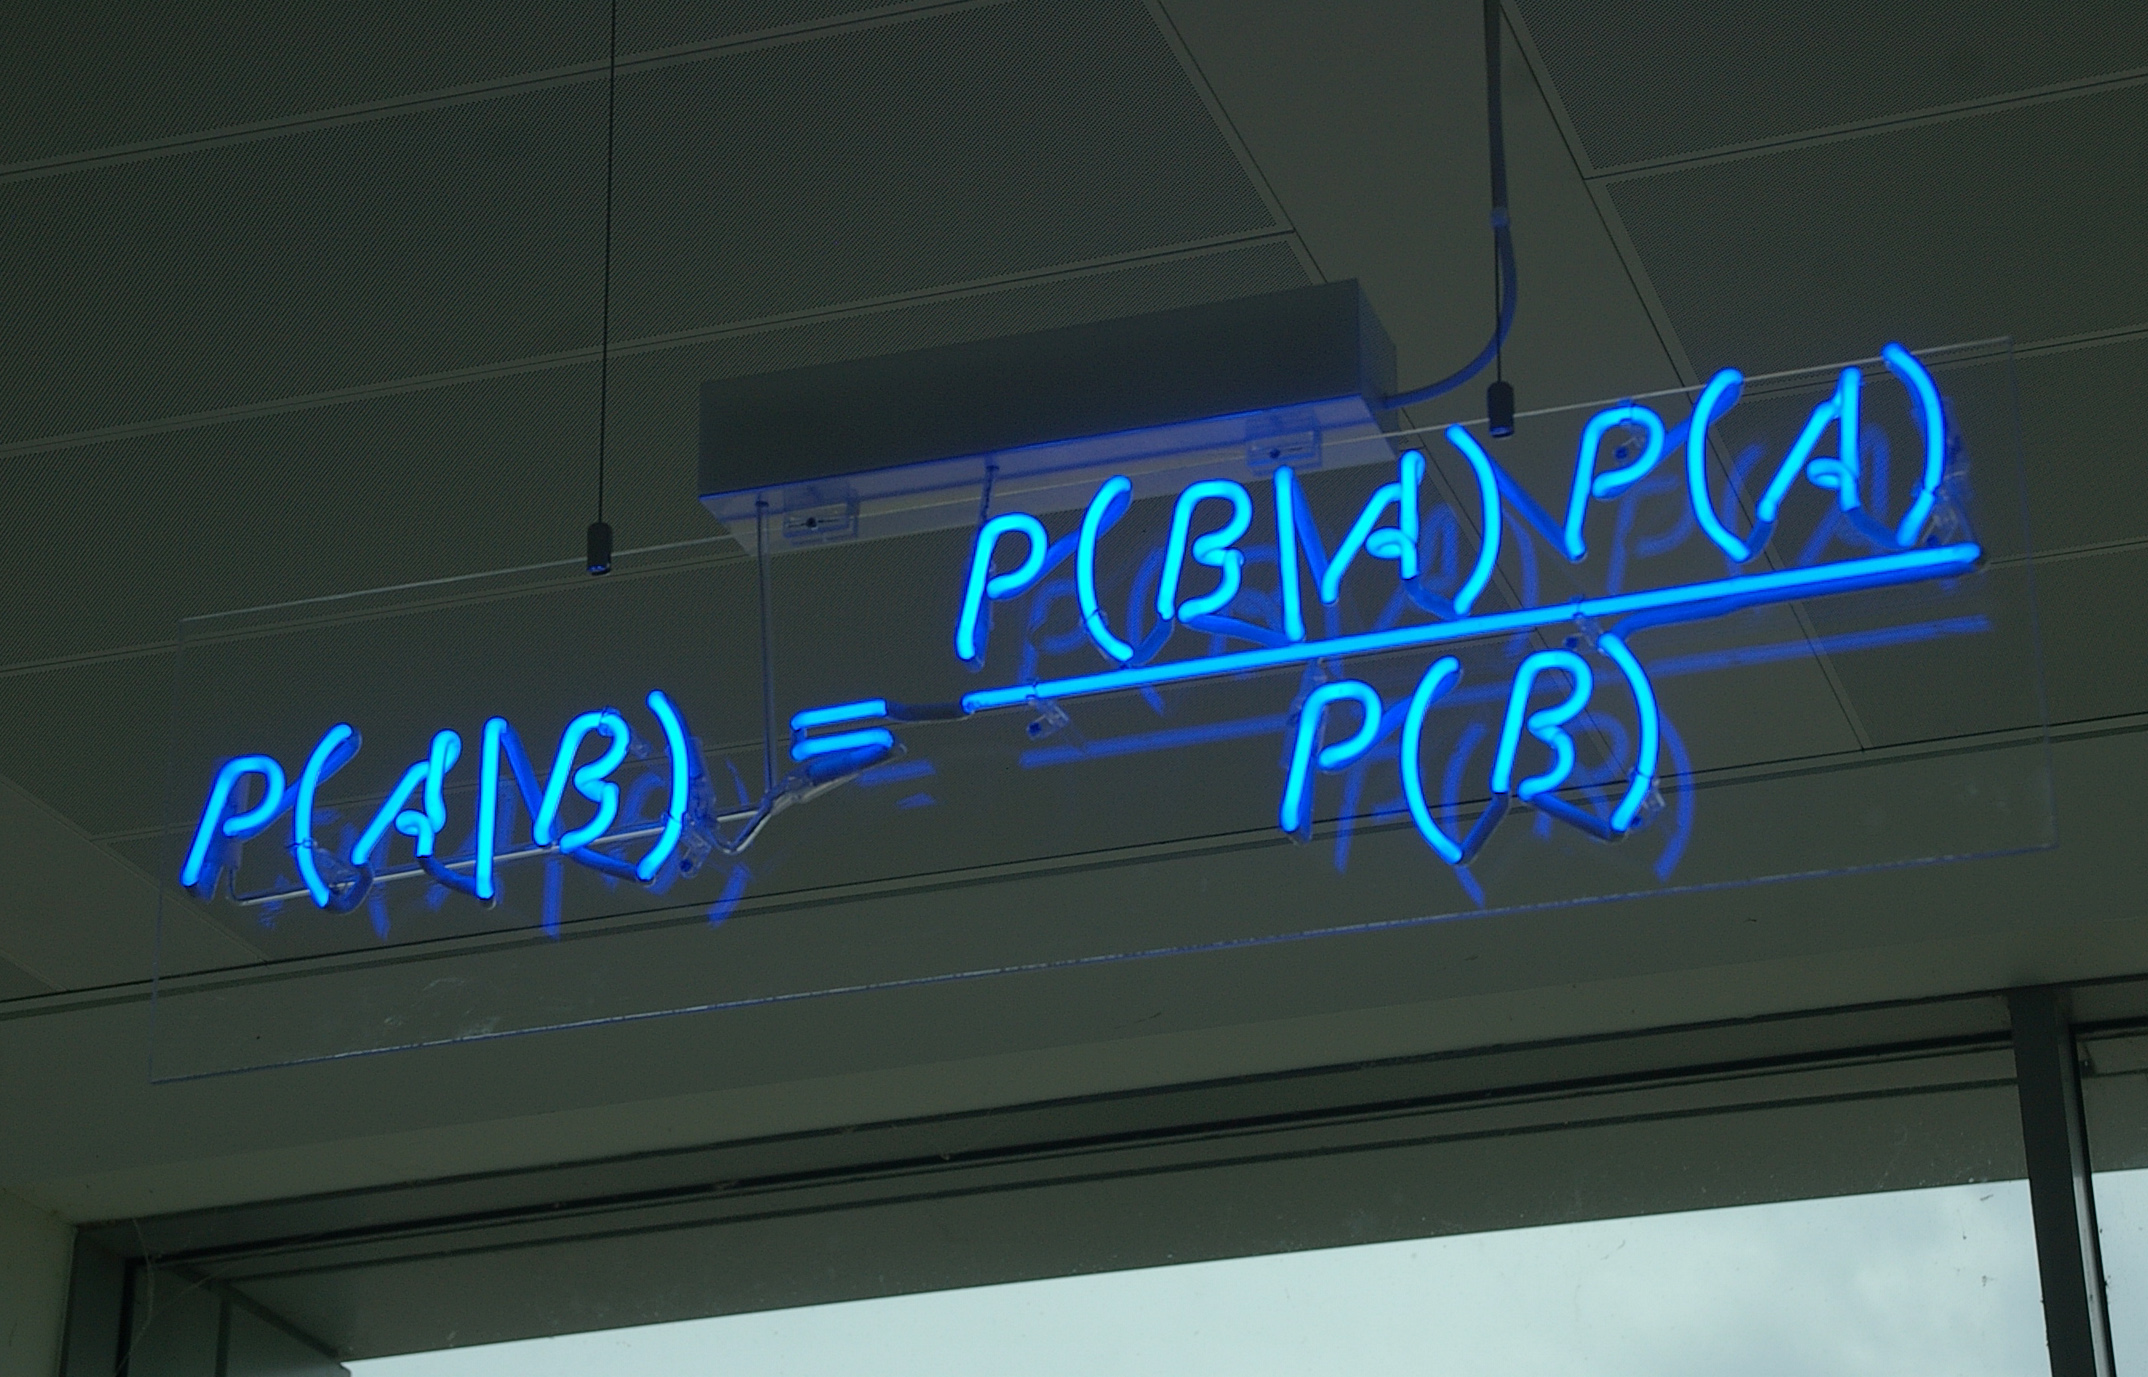
\includegraphics[scale=0.12]{./images/Bayes'_Theorem_MMB_01.jpg}
		\caption{Bayes' theorem spelt out in blue neon at the offices of Autonomy in Cambridge. (credit: \href{https://commons.wikimedia.org/wiki/User:Mattbuck}{Mattbuck, Wikipedia})}	
	\end{figure}
	
\end{frame}

\begin{frame}
	\frametitle{The exact formulation}
%	\framesubtitle{}
	Assuming we are working in a continuous space, the Bayes' Theorem can be written as:
	\begin{align}
		P(\theta | D) &= \frac{P(D | \theta) P(\theta)}{P(D)} \\
		&= \frac{P(D|\theta) P(\theta)}{\sum P(D | \theta) P(\theta)} \\
		&\propto P(D|\theta) P(\theta)
	\end{align}
	The three components of the equation are:
	\begin{itemize}
		\item $P(\theta | D)$, the posterior
		\item $P(D | \theta)$, the likelihood function
		\item $P(D)$, the normalising function
	\end{itemize}
\end{frame}

\begin{frame}
	\frametitle{The likelihood function}
%	\framesubtitle{}
	The likelihood is a function of the parameters of a statistical model given data. In other words, the likelihood describes the probability of observing the data given the parameters of the statistical model.
\end{frame}

\begin{frame}
	\frametitle{The prior distribution}
%	\framesubtitle{}
	The prior is a probabilistic formulation of our beliefs before collecting new data.
	\begin{itemize}
		\item Priors can be weak, moderate or strong, depending on how concentrated the probability density is compared to the problem space
		\item In hierarchical models, priors can be implicit, thus determined by higher level's parameters
		\item It's important to investigate priors when working with complex model because these could strongly impact the final results
	\end{itemize}

\end{frame}

\begin{frame}
	\frametitle{The posterior distribution}
%	\framesubtitle{}
	The posterior distribution is the updated belief after collecting new data.
	\begin{itemize}
		\item Could have the same form of the prior (\it{conjungancy})
	\end{itemize}
\end{frame}

\subsection{Why is Bayes' Theorem useful?}
\begin{frame}
%	\frametitle{Advantages}
%	\framesubtitle{Subtitle}
	The main reasons behind the success of Bayesian Inference are:
	\begin{itemize}
		\item It allows to account for prior knowledge, when this is relevant
		\begin{itemize}
			\item Speed-up convergence
			\item Attribute non-zero probability to yet un-observed events (contrary to frequentist approach)
		\end{itemize}
		\item Moving beyond single point estimation
		\item Estimating probability in a joint parameter space
	\end{itemize}		
\end{frame}

\subsection{A few simple examples}
\begin{frame}
%	\frametitle{The Beta-Bernoulli model}
%	\framesubtitle{}
	Empty frame
\end{frame}

\begin{frame}
%	\frametitle{The Beta-Binomial model}
%	\framesubtitle{}
	Empty frame
\end{frame}


\subsection{Data order invariance}
\begin{frame}
%	\frametitle{The Beta-Binomial model}
%	\framesubtitle{}
	Empty frame
\end{frame}


%%%%%%%%%%%%%%%%%%%%%%%%%%

\section{Moving to Bayesian Hierarchical Modelling}
\subsection{What does hierarchical/Multilevel Modelling mean?}
\begin{frame}
%	\frametitle{The Beta-Binomial model}
%	\framesubtitle{}
	Hierarchical modelling means expressing the Bayes' Theorem as depencencies between parameters instead of an expression about the joint parameter space.
	
	\begin{align}
		P(\theta, \omega | D) &= \frac{P(D | \theta, \omega) P(\theta, \omega)}{P(D)} \\
		&= \frac{P(D | \theta) P(\theta, \omega)}{P(D)} \label{eq:likelihood_ind}\\
		&= \frac{P(D | \theta) P(\theta | \omega) P(\omega)}{P(D)} \label{eq:hierarchical_formulation}
	\end{align}
	
	We made the following steps:
	\begin{itemize}
		\item \eqref{eq:likelihood_ind} because likelihood doesn't depend on $\omega$
		\item \eqref{eq:hierarchical_formulation} because $P(\theta | \omega) = \frac{P(\theta, \omega)}{P(\omega)} \text{ thus } P(\theta, \omega) = P(\theta | \omega) P(\omega)$
	\end{itemize}
\end{frame}

\begin{frame}
%	\frametitle{}
%	\framesubtitle{}
	When dealing with a continuous problem space \eqref{eq:hierarchical_formulation} becomes:
	\begin{align}
		P(\theta_1, \dots m | D) &= \frac{P(D | \theta_1, \dots m) P(\theta_1, \dots m)}{P(D)} \\
		&= \frac{P(D | \theta_1, \dots m) P(\theta_1, \dots m)}{\sum\limits_{m} \int \mathrm{d}\theta_{m} P(D | \theta_1, \dots m) P(\theta_1, \dots m)} \\
		&= \frac{\prod P_{m}(D | \theta_{m}, m) P_{m}(\theta_{m} | m) P(m)}{\sum\limits_{m} \int \mathrm{d}\theta_{m} \prod_{m} P_{m}(D | \theta_{m}, m) P_{m}(\theta_{m} | m) P(m)}
	\end{align}		
\end{frame}


\subsection{Baseball example}
\begin{frame}
%	\frametitle{The Beta-Binomial model}
%	\framesubtitle{}
	Empty frame
\end{frame}

\subsection{AdWords example}
\begin{frame}
%	\frametitle{The Beta-Binomial model}
%	\framesubtitle{}
	Empty frame
\end{frame}


%%%%%%%%%%%%%%%%%%%%%%%%%%


\section{Stan}

\subsection{A quick introduction to Stan}
\begin{frame}
%	\frametitle{The Beta-Binomial model}
%	\framesubtitle{}
	Empty frame
\end{frame}

\subsection{Working with log probability density}
\begin{frame}
%	\frametitle{The Beta-Binomial model}
%	\framesubtitle{}
	Empty frame
\end{frame}

\subsection{How to write a model in Stan}
\begin{frame}
%	\frametitle{}
%	\framesubtitle{}
	Empty frame
\end{frame}


\end{document}